\documentclass[a4paper,fleqn,12pt]{article}

\usepackage[utf8]{inputenc}
\usepackage[bulgarian]{babel}
\usepackage{amsmath}
\usepackage{amssymb}
\usepackage{booktabs}
\usepackage{fancyhdr}
\usepackage{amsthm}
\usepackage{graphicx}
\usepackage{color}
\usepackage{pdfpages}

%\pagestyle{fancy}
%\fancyhf{}
%\lhead{\rightmark}
%\rhead{\thepage}
%\cfoot{}
%\renewcommand{\headrulewidth}{0pt}

%\sloppy
%\definecolor{lightgray}{gray}{0.5}
%\setlength{\parindent}{0pt}


\begin{document}
\begin{titlepage}
	\setlength{\parindent}{0pt}
	\large
\centering
Технически университет -  София \par
Факултет по приложна математика и информатика \par
\vspace{2cm}

{\huge Курсова работа \par}

\vspace{2cm}

\vspace{1cm}
{\LARGE\scshape Математическа статистика 2 \par}



\vfill

\begin{minipage}[t]{.5\linewidth}
	Студент: \\
	Кристиян Кръчмаров
\end{minipage}%
\begin{minipage}[t]{.5\linewidth}
	\raggedleft
	Преподавател:\\
	проф. д-р Красимира Проданова
\end{minipage}

\vspace{2cm}
\raggedright

\end{titlepage}
\pagenumbering{gobble}
\tableofcontents
\newpage

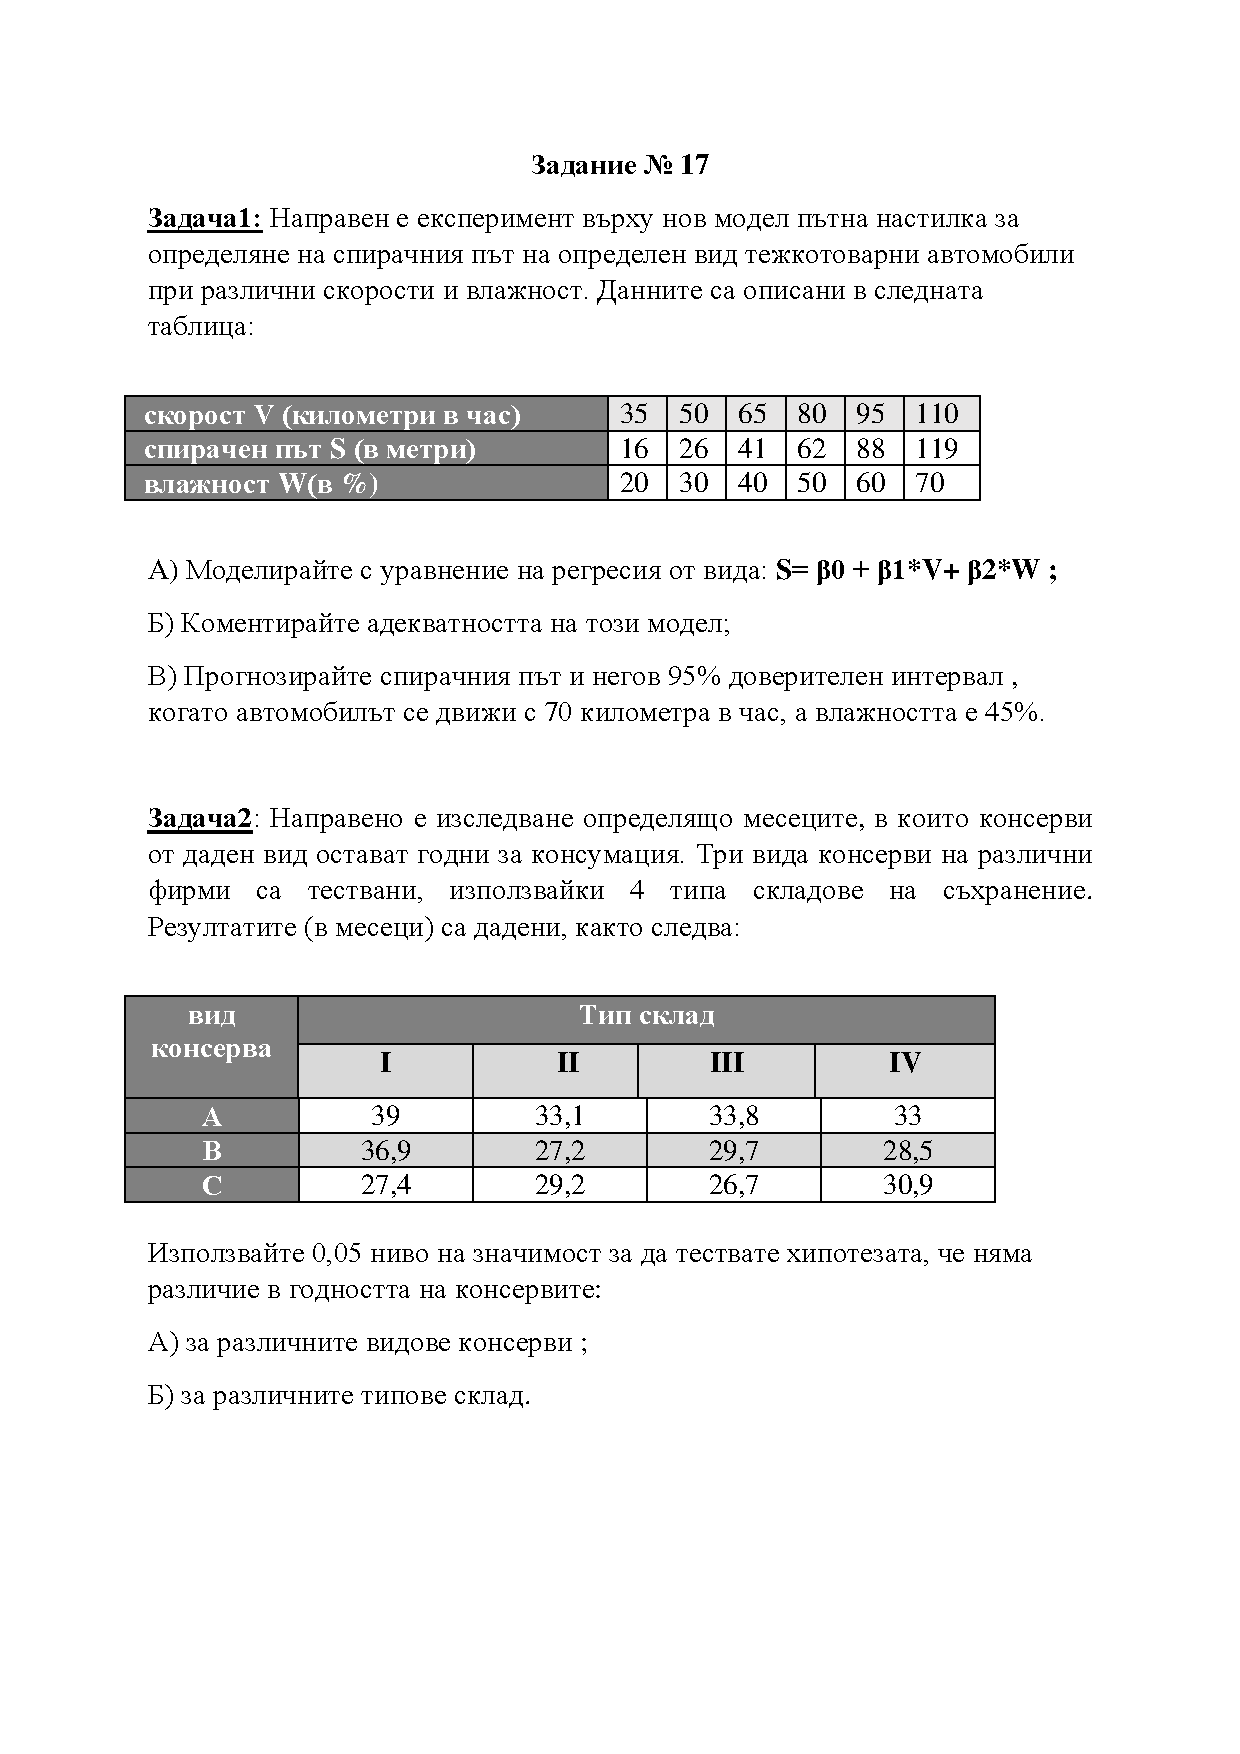
\includepdf[pages={1}]{course-work.pdf}
\newpage
\pagenumbering{arabic}
\section{Решение}
\subsection{Задача 1}

\begin{figure}[h]
  \centering
  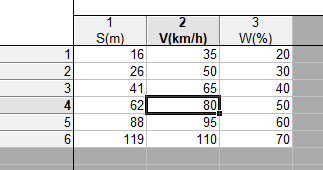
\includegraphics{task1-data.png}
  \caption{Данни}
\end{figure}
\begin{figure}[h]
  \centering
  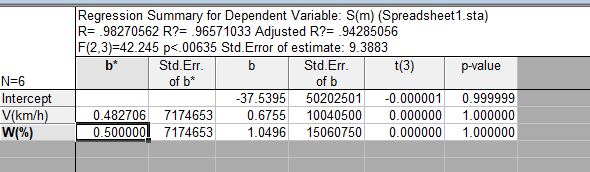
\includegraphics{task1-1.png}
  \caption{Резултати}
\end{figure}

\subsubsection{А}
$$
S = -37.5395 + 0.6755 \cdot V + 1.0496 \cdot W
$$

\subsubsection{Б}
$$
R = 0.98 \qquad R^2 = 0.96 \implies \text{ модела описва добре изходните данни}
$$

\newpage
\subsubsection{В}
\begin{figure}[htp!]
  \centering
  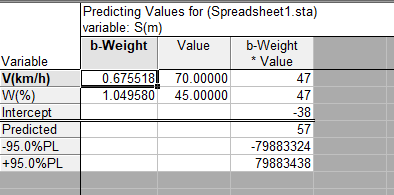
\includegraphics{task1-2.png}
  \caption{Резултати}
\end{figure}

\newpage
\subsection{Задача 2}
\begin{figure}[h]
  \centering
  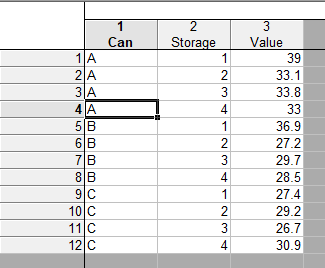
\includegraphics{task2-data.png}
  \caption{Данни}
\end{figure}

\begin{figure}[h]
  \centering
  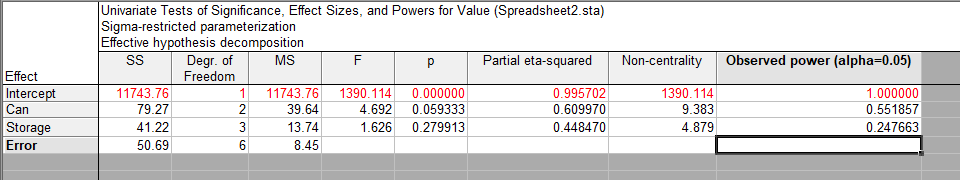
\includegraphics[width=1.2\linewidth,height= 4cm]{task2.png}
  \caption{Резултати}
\end{figure}

\subsubsection{А}
$$
p=0.059333 > 0.05 \implies \text{ има различие в годността за различните видове консерви}
$$

\subsubsection{Б}
$$
p=0.279913 > 0.05 \implies \text{ има различие в годността за различните складове}
$$






















\end{document}